\subsubsection{Criterios de Diseño}

\begin{itemize}
\bigskip 

\item  Caminos de los conductores de alimentación suficientemente anchos y  dispuestos uno próximo al otro, con el objetivo de disminuir el área efectiva y por lo tanto la impedancia.

\item Capacitores de desacople del valor adecuado, de modo que funcionen a la frecuencia correspondiente.

\item Líneas de señal generando la menor área compatible con la distribución de los elementos con su camino de retorno. Especialmente los caminos de alta corriente y/o velocidad como para líneas de gran sensibilidad.

\item Área efectiva del circuito lo más pequeña posible.

\item Conexiones de masas y alimentación sin bucles.

\item Capacidades parásitas entre masa y las líneas de señal minimizadas al alejar pistas.
\end{itemize}

\subsubsection{Circuito Implementado}

\begin{center}
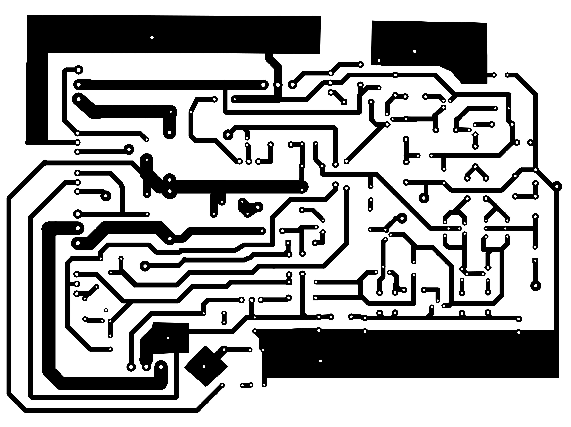
\includegraphics[scale=0.75]{img/circuito_impreso.png} 
\end{center}

